Podemos expresar un algoritmo de muchas maneras, incluyendo lenguaje natural, diagramas de flujo, pseudocódigo y diagrama NASSI – SCHNEIDERMAN.

\subsection{Lenguaje natural}
El lenguaje natural es popular, pues se nos da naturalmente y puede comunicar los pasos de un algoritmo a una audiencia general. Cuando desarrollamos algoritmos, a menudo trabajamos con personas que saben programación y con algunos que no; pero todos conocen el lenguaje natural.

Sin embargo, el lenguaje natural tiene inconvenientes. Tiende a ser ambiguo y a estar definido vagamente, pues carece de estructura precisa. Esto dificulta que otros sigan un algoritmo y se sientan seguros de que es correcto. Los diagramas de flujo y el pseudocódigo son formatos más estructurados que pueden expresar un algoritmo de manera más precisa, y son populares con científicos de computación y programadores.

\subsection{Diagramas de flujo}

Una manera más formal de expresar un algoritmo es con un diagrama de flujo, un diagrama con cajas conectadas por flechas.

% TODO: \usepackage{graphicx} required
\begin{figure}[h!]
	\centering
	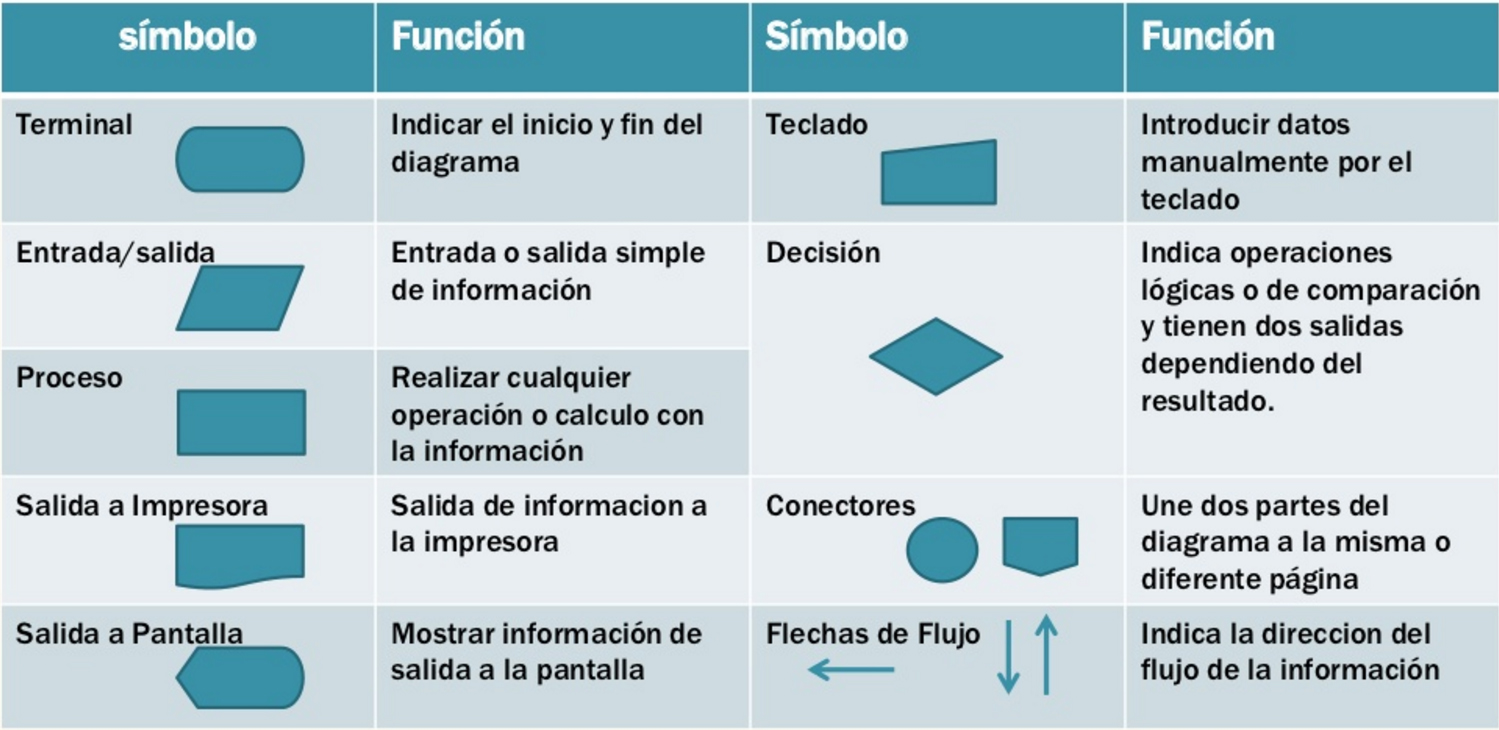
\includegraphics[width=0.9\linewidth]{img/simbolos_diagrama}
	\label{fig:simbolosdiagrama}
\end{figure}

\textbf{Objetivos del diagrama de flujo}

\begin{itemize}
	\item Ofrecer una descripción visual de las actividades implicadas en un proceso mostrando la relación secuencial ente ellas.
	\item Facilitar la rápida comprensión de cada actividad y su relación con las demás, el flujo de la información, las ramas en el proceso, el número de pasos del proceso, etc. 
	\item Facilitar la selección de indicadores de proceso. 
	\item Estimula el pensamiento analítico en el momento de estudiar un proceso, haciendo más factible generar alternativas útiles. 
\end{itemize}


Expresar un algoritmo como un diagrama de flujo nos permite visualizar el algoritmo a nivel alto, además de que nos obliga a pensar muy cuidadosamente en la secuenciación y selección. ¿Cuál flecha va a cuál nodo? ¿Faltan flechas? Estos son los tipos de preguntas valiosas que pueden surgir al traducir un algoritmo a un diagrama de flujo.

\subsection{Pseudocódigo}

Finalmente la mayoría de los algoritmos se transforman en código para ejecutar en una computadora. Antes de eso, los programadores a menudo prefieren expresar un algoritmo en pseudocódigo: un código que utiliza construcciones de un lenguaje de programación, pero que en realidad, no se ejecuta. 

Cada programador escribe pseudocódigo de manera diferente, pues no hay un estándar oficial, así que puedes toparte con pseudo-código que se vea muy diferente. 

Expresar un algoritmo en pseudocódigo ayuda a un programador a pensar en términos familiares, sin preocuparse por la sintaxis y detalles específicos. También le provee a los científicos de computación una forma independiente del lenguaje para expresar un algoritmo, de manera que los programadores de cualquier lenguaje puedan tomarla, leer el pseudo-código y traducirlo a su lenguaje favorito.

Escribir en pseudocódigo es similar a escribir en un lenguaje de programación. Cada paso del algoritmo está escrito en una línea propia en secuencia. Por lo general, instrucciones se escriben en mayúsculas ,variables en minúsculas y mensajes en mayúsculas y minúsculas

Al escribir pseudocódigo, todos suelen tener su propio estilo de presentar las cosas, ya que lo leen los humanos y no una computadora. sus reglas son menos rigurosas que las de un lenguaje de programación. Sin embargo, hay algunas reglas simples que ayudan a que el pseudocódigo sea más universalmente entendido.

\textbf{Reglas para escribir pseudocódigo}

\begin{itemize}
	\item Siempre escribe en mayúscula la palabra inicial (a menudo una de las 6 construcciones principales).
	\item Tener sólo una declaración por línea.
	\item Aplicar sangría para mostrar jerarquía, mejorar la legibilidad y mostrar construcciones anidadas.
	\item Finaliza siempre las secciones de varias líneas con cualquiera de las palabras clave END ( ENDIF , ENDWHILE , etc.).
	\item Mantén tus declaraciones independientes del lenguaje de programación.
	\item Mantenlo simple , conciso y legible .
\end{itemize}

Una de las ventajas que presenta esta forma de representación de algoritmos es que facilita mucho su escritura posterior en un lenguaje de programación y le permite al diseñador aprender de una manera más sencilla debido a su familiaridad con cualquier lenguaje de programación.

Otra ventaja con que se cuenta, es que es independiente de la plataforma o lenguaje de programación que se desee utilizar, ya que su escritura no implica palabras reservadas de ningún tipo de lenguaje.

\subsection{Diagrama NASSI – SCHNEIDERMAN}

Conocido como diagrama N-S, se considera como otra forma de representar algoritmos. Se basa en escribir las instrucciones en bloques o cuadros de texto. Este diagrama también se conoce con el nombre de diagrama de Chapin y es una combinación de la escritura en pseudocódigo y del diagrama de flujo.

En el diagrama N-S, las flechas que indican el flujo del algoritmo, se reemplazan por las cajas de texto, en las cuales se escriben las instrucciones respectivas.

% TODO: \usepackage{graphicx} required
\begin{figure}[!h]
	\centering
	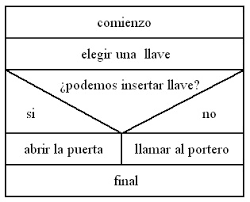
\includegraphics[width=0.4\linewidth]{img/Diagrama_NASSI_SCHNEIDERMAN}
	\label{fig:diagramanassischneiderman}
\end{figure}


Como se puede apreciar, cada bloque contiene una instrucción, en el caso de definición de variables, se recomienda utilizar un bloque por cada tipo de datos distinto que se genere, es decir si existen varios datos enteros, su definición abarcaría un solo bloque, si por el contrario se requieren definir datos dobles, ellos ocuparían otro bloque y así sucesivamente.

Las principales desventajas de este diagrama radica en si el algoritmo es demasiado largo, este tipo de diagrama es difícil de realizar y consume bastante tiempo de elaboración dos elementos muy importante a tener en cuenta ya que en las soluciones a problemas algunos de los algoritmos pueden ser largos y no podemos perder mucho tiempo en la elaboración ya que en una competencia el factor tiempo es importante.
